\documentclass[english,compress]{beamer}

\usepackage{tcolorbox}
\usepackage{listings}
\newcommand{\cw}{\texttt} % to display a word as in code format
\setbeamertemplate{section page}
{
	\begin{centering}
	\begin{beamercolorbox}[sep=12pt,center]{part title}
	\usebeamerfont{section title}\insertsection\par
	\end{beamercolorbox}
	\end{centering}
}
\tcbuselibrary{listings}
\useoutertheme{split}
\useinnertheme{rectangles}
\usecolortheme{uiuc}
\logo{
\includegraphics[height=0.5cm]{uiuclogo.pdf}}
\AtBeginSection{\frame{\sectionpage}}

\title{SIAM: Getting Started with Git}
\subtitle{based on http://git-scm.com/book and slides by Bart Trojanowski}
\author{Andrew Reisner and Nathan Bowman}
\date{\today}

\begin{document}
\frame{\titlepage}
\frame{\frametitle{Table of Contents}\tableofcontents}

\section{Overview}
\frame
{
    \frametitle{Git}
    \begin{columns}
    \begin{column}{.5\textwidth}
        Git is a
        \begin{itemize}
            \item Free and Open Source
            \item Distributed
            \item Version Control System.
        \end{itemize}
    \end{column}
    \begin{column}{.5\textwidth}
        \begin{center}
            
\includegraphics[width=.7\textwidth]{figs/git-logo.png} 
        \end{center}
    \end{column}
    \end{columns}
}

\frame
{
    \frametitle{Version Control System}

        Preserve a clear, timely record of software evolution
            \begin{itemize}
                \item Record changes to files
                \item History can be recalled/inspected
            \end{itemize}
        Implications:
            \begin{itemize}
                \item Rollback changes
                \item Know what collaborators are working on
                \item Investigate changes when bugs emerge
                \item Find how and where a particular bug was fixed
            \end{itemize}
}

\section{Components}
\frame
{
    \frametitle{VCS Components (Working Tree)}

    \begin{itemize}
        \item Single checkout of one version of the project
        \item Directories
        \item Files
    \end{itemize}
    \begin{center}
        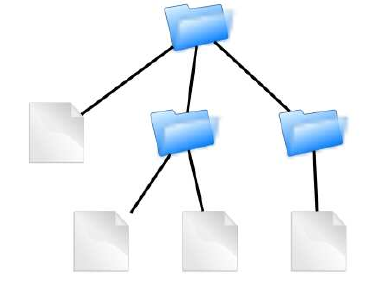
\includegraphics[height=.3\textwidth]{figs/working-tree.png}
    \end{center}
}

\frame
{
    \frametitle{VCS Components (Repository)}

    \begin{columns}
        \begin{column}{.5\textwidth}
    \begin{itemize}
        \item Files
        \item Commits
        \item Ancestry
    \end{itemize}
\end{column}
\begin{column}{.5\textwidth}
    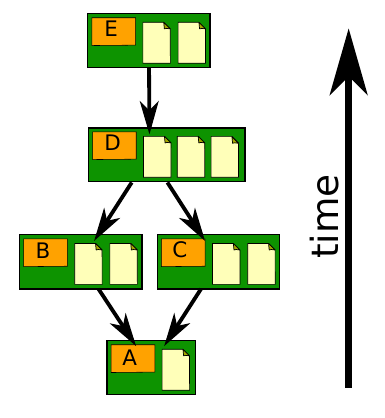
\includegraphics[width=.8\textwidth]{figs/repo.png}
\end{column}
\end{columns}
}

\frame
{
    \frametitle{VCS Components (References)}

    \begin{columns}
        \begin{column}{.5\textwidth}
    \begin{itemize}
        \item Tags
        \item Branches
        \item \cw{HEAD}
        \item Index (Staging area)
    \end{itemize}
\end{column}
\begin{column}{.5\textwidth}
    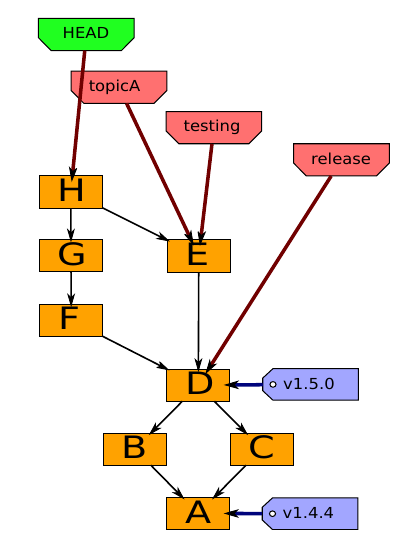
\includegraphics[width=\textwidth]{figs/references.png}
\end{column}
\end{columns}
}

\section{Operations}
\frame
{
    \frametitle{VCS Operations}
        \begin{columns}
            \begin{column}{.5\textwidth}
        Bootstrap
            \begin{itemize}
                \item \cw{init}
                \item \cw{clone}
                \item \cw{checkout}
            \end{itemize}
        Modify
        \begin{itemize}
            \item \cw{add}, delete (\cw{rm})
			\item rename (\cw{mv})
            \item \cw{commit}
        \end{itemize}
         Information
        \begin{itemize}
            \item \cw{status}
            \item \cw{diff}
            \item \cw{log}
        \end{itemize}
   \end{column}
    \begin{column}{.5\textwidth}
        Reference
        \begin{itemize}
            \item \cw{tag}
            \item \cw{branch}
        \end{itemize}
        Sharing work, backing it up
\begin{itemize}
    \item \cw{pull}, \cw{fetch}
    \item \cw{push}
\end{itemize}

    \end{column}
\end{columns}

}
\frame
{
    \begin{center}
        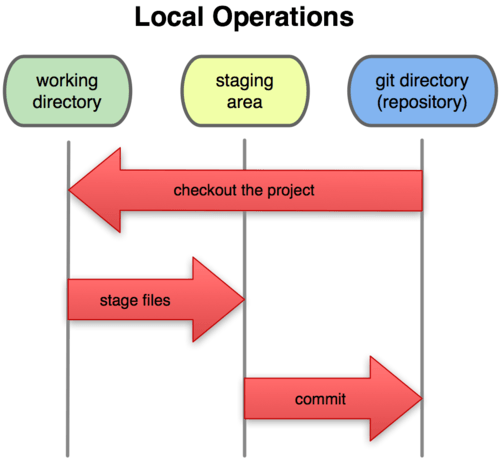
\includegraphics[width=.8\textwidth]{figs/sections.png}
    \end{center}
}

\subsection{Creating and Updating}
\begin{frame}[fragile]
    \frametitle{Bootstrapping}
    
    \verb|$ git init|
    \begin{itemize}
        \item creates .git directory and initializes the repository
    \end{itemize}
    \verb|$ git clone <URL>|
    \begin{itemize}
        \item replicates a remote repository
        \item checks out new working tree
        \item Git URLs
            \begin{itemize}
                \item /home/user/my-project.git
                \item http://github.com/user/my-project.git
                \item git://remote.server/my-project.git
                \item user@remote.server:my-project.git
                \item ssh://user@remote.server/~user/my-project.git
            \end{itemize}
    \end{itemize}
\end{frame}

\begin{frame}[fragile]
    \frametitle{Staging}
    \verb|$ git add <path>|
    \begin{itemize}
        \item Adds contents of \verb|<path>| to index
        \item \verb|$ git add .|
    \end{itemize}
    
    \verb|$ git rm <file>|
    \begin{itemize}
        \item Removes files from working tree and index
    \end{itemize}

    \verb|$ git mv <source> <destination>|
    \begin{itemize}
        \item Moves or renames a file or directory
    \end{itemize}
    \verb|.gitignore|
    \begin{itemize}
        \item Text file that specifies files to ignore
    \end{itemize}
\end{frame}

\begin{frame}[fragile]
    \frametitle{Example \cw{.gitignore} file}

    \begin{tcblisting}{listing only}
*.aux
*.fdb_latexmk
*.fls
*.nav
*.out
*.snm
*.toc
*.vrb
*~
    \end{tcblisting}
\end{frame}

\begin{frame}[fragile]
    \frametitle{Changing Settings}

	\verb|$ git config --list|
	\begin{itemize}
		\item Lists the current configuration settings
	\end{itemize}
	\verb|$ git config <key>|
	\begin{itemize}
		\item Gets the current value of \verb|key|
	\end{itemize}
	\verb|$ git config [level] <key> <value>|
	\begin{itemize}
		\item Changes setting \verb|key| to \verb|value|
		\item Optional \verb|level| determines scope of setting
		\begin{itemize}
			\item Omitting \verb|level|: repository
			\item \verb|--global|: user
			\item \verb|--system|: system
		\end{itemize}
	\end{itemize}
\end{frame}

\begin{frame}[fragile]
    \frametitle{Common Configuration Settings}
	A few settings you will want to update when first using Git:\\ \ \\
	\verb|$ git config --global user.name "John Doe"|
	\verb|$ git config --global user.email johndoe@example.com|
	\verb|$ git config --global core.editor emacs|
	\verb|$ git config --global core.excludesfile ~/.gitignore|
	\verb|$ git config --global merge.tool meld|
\end{frame}

\begin{frame}[fragile]
    \frametitle{Committing}

    \verb|$ git commit -m <msg>|
    \begin{itemize}
        \item Creates a commit of staged items
        \item \verb|$ git commit -m "fixes issue #108"|
    \end{itemize}
\end{frame}

\subsection{Getting Information}
\begin{frame}[fragile]
    \frametitle{Inspection}

    \verb|$ git status|
    \begin{itemize}
        \item Displays the working tree status
        \item staged, unstaged, untracked
    \end{itemize}
    \verb|$ git diff|
    \begin{itemize}
        \item Displays changes between index and working tree
    \end{itemize}
    \verb|$ git diff --staged|
    \begin{itemize}
        \item Displays changes between HEAD and index
    \end{itemize}
    \verb|$ git diff HEAD|
    \begin{itemize}
        \item Displays changes between HEAD and working tree
    \end{itemize}
    \verb|$ git diff <commit> <commit>|
    \begin{itemize}
        \item Displays changes between two commits
    \end{itemize}
\end{frame}

\begin{frame}[fragile]
    \frametitle{Demonstration of Staging}
    \begin{tcblisting}{listing only}
$ echo "foo" >> myfile
$ git diff myfile
diff --git a/myfile b/myfile
index e69de29..257cc56 100644
--- a/myfile
+++ b/myfile
@@ -0,0 +1 @@
+foo
    \end{tcblisting}
\end{frame}

\begin{frame}[fragile]
    \frametitle{Referencing Objects}

    \begin{itemize}
        \item \verb|a88dbbe57b9e9fc01f701c45c405647c588e6a6a|
        \item \verb|a88d|
        \item \verb|v1.0.3|
        \item \verb|master|
        \item \verb|origin/master|
        \item \verb|HEAD|
        \item \verb|HEAD^ == HEAD~1|
        \item \verb|feature_brach@{May.30}|
    \end{itemize}
\end{frame}

\begin{frame}[fragile]
    \frametitle{Show and Log}

    \verb|$ git show <object>|
    \begin{itemize}
        \item Show various types of objects
        \item \verb|$ git show HEAD@{yesterday}|
        \item \verb|$ git show HEAD:file|
    \end{itemize}

    \verb|$ git log [<since>..<until>] [-- <path>]|
    \begin{itemize}
        \item Show commit logs
        \item \verb|$ git log HEAD~3..HEAD^|
        \item \verb|$ git log -- file-with-bug.c|
    \end{itemize}
\end{frame}

\subsection{Branching and Remotes}
\begin{frame}[fragile]
    \frametitle{Branching}

    \verb|$ git branch -l|
    \begin{itemize}
        \item List local branches
    \end{itemize}

    \verb|$ git branch <branchname> |
    \begin{itemize}
        \item Create new branch on HEAD
    \end{itemize}

    \verb|$ git branch <branchname> <start-commit>|
    \begin{itemize}
        \item Create new branch on specified commit
    \end{itemize}

    \verb|$ git checkout <branch>|
    \begin{itemize}
        \item Checkout branch by name
    \end{itemize}

    \verb|$ git checkout -b <branchname> [<start-commit>]|
    \begin{itemize}
        \item Create and switch to a new branch
    \end{itemize}
\end{frame}

\begin{frame}[fragile]
    \frametitle{Merging}

    \verb|$ git merge <branch>|
    \begin{itemize}
        \item Incorporates changes from the specified branch into the current
            branch.
        \item Conflicts may result
        \item Any conflicts must be resolved before merge is completed
    \end{itemize}

    \begin{tcblisting}{listing only}
var = 3
<<<<<<< HEAD
x = 0.5 * var
=======
x = 1/2. * var
>>>>>>> origin/master
    \end{tcblisting}
\end{frame}

\begin{frame}[fragile]
    \frametitle{Mergetool}

    \verb|$ git merge <branch>|
    \begin{itemize}
        \item Presents a visual interface to merging
        \item Example: 
		\item \verb|$ git mergetool --tool=meld|
    \end{itemize}
    \begin{center}
        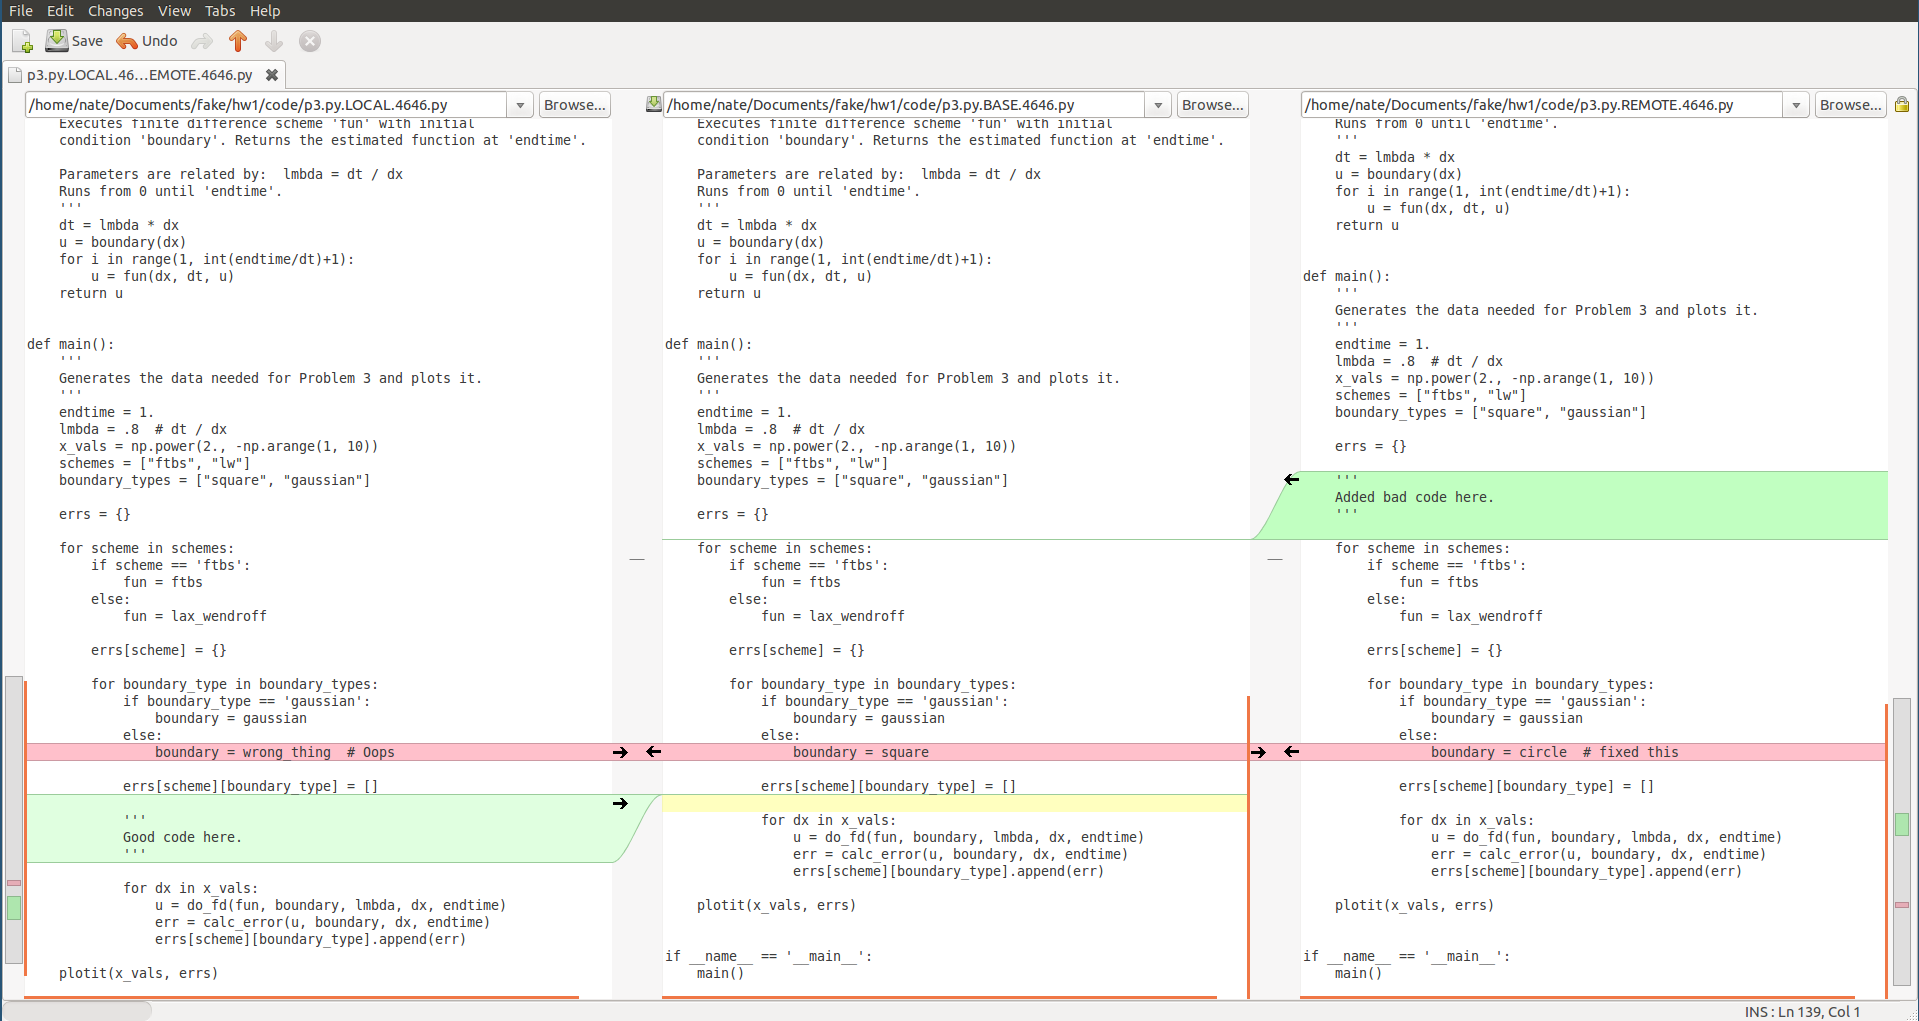
\includegraphics[width=.9\textwidth]{figs/meld_screenshot}
    \end{center}

\end{frame}

\begin{frame}[fragile]
    \frametitle{Remotes}

    \verb|$ git remote add <name> <url>|
    \begin{itemize}
        \item Adds a remote named \verb|<name>| for the repository at \verb|<url>|
    \end{itemize}

    \verb|$ git fetch <remote>|
    \begin{itemize}
        \item Fetches updates from specified remote
        \item \verb|$ git fetch --all|
    \end{itemize}

    \verb|$ git branch -r |
    \begin{itemize}
        \item List remote branches
        \item Use \verb|$ git merge| to merge these branches
    \end{itemize}

    \verb|$ git pull [<remote>] [<branch>]|
    \begin{itemize}
        \item Short for a fetch followed by a merge
    \end{itemize}
\end{frame}

\begin{frame}[fragile]
    \frametitle{Challenge Problem}

    Shape module at \verb|https://github.com/dattashantih/git-example.git|
    \begin{itemize}
        \item Fork and clone repository
        \item Locate and fix bug
        \item Push to your public repository
        \item Submit pull request (note: pull requests will be processed in 
            order and must be up to date)
    \end{itemize}
\end{frame}

\section{Distributed Workflows}
\frame
{
    \frametitle{Distributed}
    \begin{itemize}
        \item No central location that keeps track of your data (no single place is more important than another)
        \item Encourages small commits and frequent merging
        \item Branches don't affect the main repository and can commit changes without disturbing others
        \item Work offline
        \item Rely on a network of trust
    \end{itemize}
}

\frame
{
    \frametitle{Distributed Workflows: Centralized}

    \begin{center}
        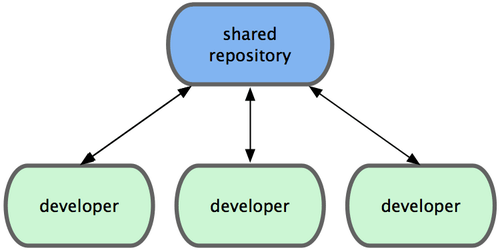
\includegraphics[width=.7\textwidth]{figs/centralized-workflow.png}
    \end{center}
}

\frame
{
    \frametitle{Distributed Workflows: Integration-Manager}

    \begin{center}
        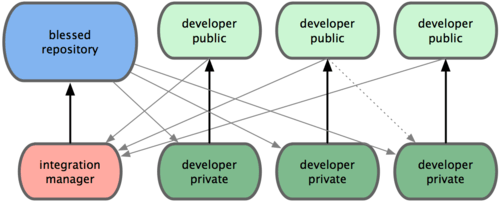
\includegraphics[width=.7\textwidth]{figs/integration-manager-workflow.png}
    \end{center}

}

\frame
{
    \frametitle{Distributed Workflows: Dictator and Lieutenants}

    \begin{center}
        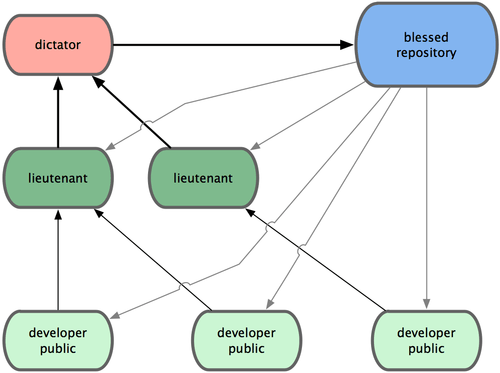
\includegraphics[width=.7\textwidth]{figs/dictator-lieutenant-workflow.png}
    \end{center}

}

\section{Git on the Web}
\frame
{
    \frametitle{Free and Open Source}

    \begin{itemize}
        \item Downloads at \url{http://git-scm.com}
        \item Libgit2: free and open source library for writing custom Git applications
        \begin{columns}
            \begin{column}{.5\textwidth}
                \begin{center}
                    
\includegraphics[width=1\textwidth]{figs/git-logo1.png}
                \end{center}
            \end{column}
            \begin{column}{.5\textwidth}
                \begin{center}
                    
\includegraphics[width=1\textwidth]{figs/libgit-logo.png}
                \end{center}
            \end{column}
        \end{columns}
    \end{itemize}
}

\frame
{
    \frametitle{GitHub}

    \begin{itemize}
        \item Powerful web interface for publishing Git repositories
        \item Simple to view changes and track progress on repositories
        \item Wiki and bug tracking built into each repository 
    \end{itemize}
    
    \begin{center}
        
\includegraphics[width=.8\textwidth]{figs/github-logo.png}
    \end{center}
}

\frame
{
    \frametitle{Bitbucket}

    \begin{itemize}
        \item Similar to GitHub
        \item Allows private repositories for students
    \end{itemize}
    
    \begin{center}
        
\includegraphics[width=.8\textwidth]{figs/bitbucket-logo.png}
    \end{center}
}

\frame
{
\small
    \frametitle{Resources}
    \begin{enumerate}
        \item Git From the Bottom Up\\
            \url{http://ftp.newartisans.com/pub/git.from.bottom.up.pdf}
        \item User Manual\\
            \url{http://git-scm.com/docs/user-manual.html}
        \item Git Magic\\
            \url{http://www-cs-students.stanford.edu/~blynn/gitmagic/}
        \item Git Book\\
            \url{http://git-scm.com/book}
        \item Tech Talk: Linus Torvalds on git\\
            \url{http://youtu.be/4XpnKHJAok8} 
        \item Code School - Try Git\\
            \url{http://try.github.io}
    \end{enumerate}
}
\end{document}
